% figure1_chipflow_v1.tex — chipflow round 3 (semantic + compile fixes).
% (a) pikv workflow (unchanged) — internal score/top-K/promote subtitle stays.
% (b) shows the MECHANISM via concrete chips, NOT a duplicate operator pipeline:
%   - Host before: ALL orange (no pre-highlighted candidates).
%   - RepairKV pill: a single labeled box. Score/top-K/promote happen INSIDE
%     it implicitly; (a)'s subtitle already names them.
%   - Host after: same 4x6 grid, with 3 ghost-outlined empty slots showing
%     which positions were promoted (chosen AFTER scoring inside RepairKV).
%   - GPU after: same 5 blue + 3 teal appended (the promoted entries).
%   - Symmetric cell widths, centered pill, signal s clearly outside pill.
% Shared preamble for standalone Figure 1 variants.
\documentclass[border=8pt,tikz]{standalone}
\usepackage{amsmath}
\usepackage{amssymb}
\usepackage{tikz}
\usetikzlibrary{arrows.meta,positioning,calc,fit,shapes.geometric,backgrounds}
\usepackage{xcolor}
\usepackage[T1]{fontenc}
\usepackage{mathptmx}
\newcommand{\repairkv}{\textsc{RepairKV}}
\newcommand{\bbase}{\ensuremath{B_{\mathrm{base}}}}
\newcommand{\bmatch}{\ensuremath{B_{\mathrm{match}}}}

\begin{document}
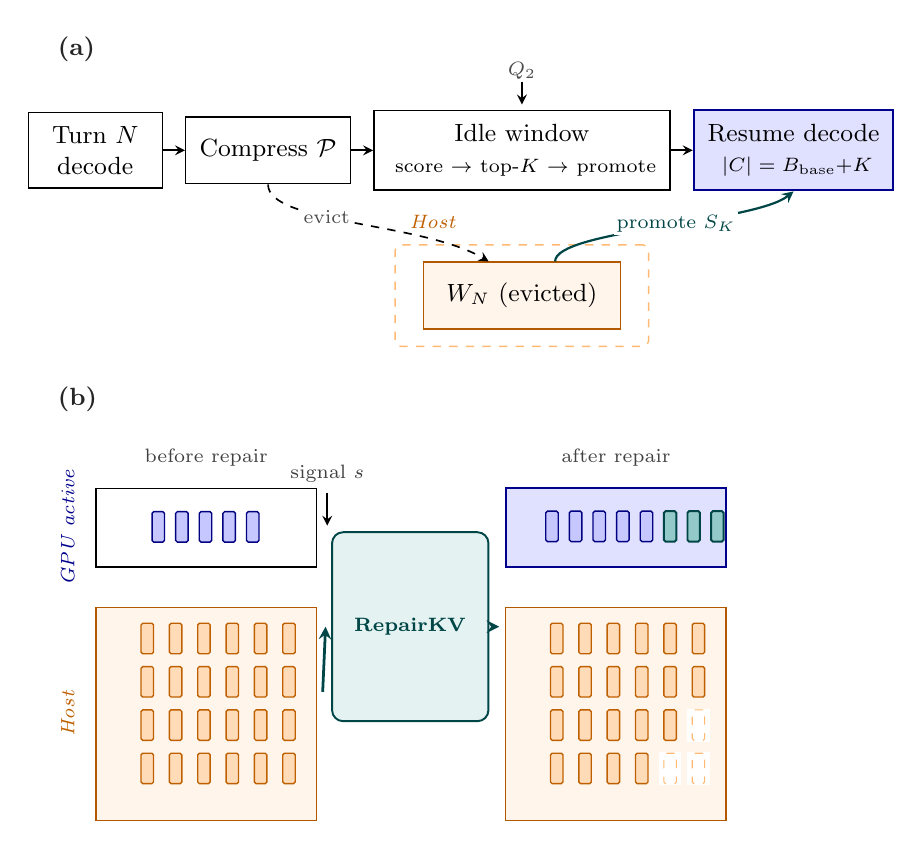
\begin{tikzpicture}[
  >=latex, line width=0.4pt,
  font=\small,
  box/.style={draw=black, fill=white, line width=0.5pt,
              inner sep=5pt, align=center, minimum height=0.85cm},
  active/.style={box, fill=blue!12, draw=blue!55!black, line width=0.7pt},
  store/.style={box, fill=orange!8, draw=orange!70!black},
  arr/.style={->, line width=0.6pt, draw=black, >=stealth},
  promarr/.style={->, line width=0.8pt, draw=teal!55!black, >=stealth},
  arrlabel/.style={font=\scriptsize, text=black!70, fill=white, inner sep=1pt},
  groupbox/.style={draw=orange!55, dashed, line width=0.5pt, rounded corners=2pt},
  grouplabel/.style={font=\scriptsize\itshape, text=orange!75!black},
  panellabel/.style={font=\bfseries\small, text=black!85},
  chip/.style={rounded corners=0.6pt, minimum width=4.5pt, minimum height=11pt,
               inner sep=0pt, line width=0.5pt},
  ghostchip/.style={chip, draw=orange!55, fill=white, dashed, line width=0.4pt},
  gpuchip/.style={chip, draw=blue!50!black, fill=blue!22},
  hostchip/.style={chip, draw=orange!75!black, fill=orange!28},
  promchip/.style={chip, draw=teal!55!black, fill=teal!42, line width=0.7pt},
  rkvpill/.style={draw=teal!55!black, fill=teal!10, line width=0.7pt,
                  rounded corners=4pt, inner sep=8pt, align=center,
                  font=\scriptsize\bfseries, text=teal!55!black,
                  minimum width=1.5cm, minimum height=2.0cm},
  rowlabel/.style={font=\itshape\scriptsize},
  bigpromarr/.style={->, line width=1.0pt, draw=teal!55!black, >=stealth}
]
  % =================================================================
  % Panel (a) — pikv block diagram
  % =================================================================
  \node[panellabel, anchor=south west] at (0, 4.4) {(a)};

  \node[box, minimum width=1.7cm] (dN) at (0.6, 3.4) {Turn $N$\\decode};
  \node[box, minimum width=1.6cm, right=8pt of dN] (cmp) {Compress~$\mathcal{P}$};
  \node[box, minimum width=2.5cm, right=8pt of cmp] (idle)
       {Idle window\\{\scriptsize{} score~$\to$~top-$K$~$\to$~promote}};
  \node[active, minimum width=1.9cm, right=8pt of idle] (resume)
       {Resume decode\\{\scriptsize{} $|C|=\bbase{+}K$}};

  \draw[arr] (dN) -- (cmp);
  \draw[arr] (cmp) -- (idle);
  \draw[arr] (idle) -- (resume);

  \draw[arr] ([yshift=10pt]idle.north) -- ([yshift=2pt]idle.north);
  \node[arrlabel, anchor=south] at ([yshift=10pt]idle.north) {$Q_2$};

  \node[store, minimum width=2.5cm, below=0.9cm of idle] (wn) {$W_N$ (evicted)};
  \node[groupbox, fit=(wn), inner xsep=10pt, inner ysep=6pt] (hgroup) {};
  \node[grouplabel, anchor=south west]
       at ([xshift=2pt, yshift=2pt]hgroup.north west) {Host};

  \draw[arr, dashed]
       (cmp.south) .. controls ([yshift=-0.5cm]cmp.south)
                              and ([yshift=0.5cm]wn.north west) ..
       ([xshift=-12pt]wn.north)
       node[arrlabel, pos=0.4] {evict};

  \draw[promarr]
       ([xshift=12pt]wn.north) .. controls ([xshift=12pt, yshift=0.4cm]wn.north)
                                          and ([xshift=-0.5cm, yshift=-0.4cm]resume.south) ..
       (resume.south)
       node[arrlabel, text=teal!55!black, pos=0.55] {promote~$S_K$};

  % =================================================================
  % Panel (b) — concrete-chip mechanism (NOT a duplicate operator pipeline)
  %   Equal-width before/after cells, centered RepairKV pill, ghost slots
  %   in host_after at promoted positions.
  % =================================================================
  \node[panellabel, anchor=south west] at (0, -0.05) {(b)};

  \node[box,    minimum width=2.8cm, minimum height=1.0cm,
        anchor=south west] (gpuB) at (0.6, -1.9) {};
  \node[active, minimum width=2.8cm, minimum height=1.0cm,
        anchor=south west] (gpuA) at (5.8, -1.9) {};
  \node[store,  minimum width=2.8cm, minimum height=2.7cm,
        anchor=north west] (hostB) at (0.6, -2.4) {};
  \node[store,  minimum width=2.8cm, minimum height=2.7cm,
        anchor=north west] (hostA) at (5.8, -2.4) {};

  % Tier row labels
  \node[rowlabel, text=blue!55!black, anchor=south, rotate=90]
       at ([xshift=-4pt]gpuB.west) {GPU active};
  \node[rowlabel, text=orange!75!black, anchor=south, rotate=90]
       at ([xshift=-4pt]hostB.west) {Host};

  % Column titles (regular weight, like (a))
  \node[font=\scriptsize, text=black!75, anchor=south]
       at ([yshift=4pt]gpuB.north) {before repair};
  \node[font=\scriptsize, text=black!75, anchor=south]
       at ([yshift=4pt]gpuA.north) {after repair};

  % --- Single RepairKV pill, centered between cells, on GPU/Host divider ---
  % Pill at x=4.6, y center = -2.15 (midpoint of -1.9 GPU bottom and -2.4 Host top).
  \node[rkvpill, minimum width=1.4cm, minimum height=2.4cm,
        anchor=center] (rkv) at (4.6, -2.65) {\repairkv{}};

  % Signal s: short downward arrow OUTSIDE the pill (above-left)
  \draw[arr] ([xshift=-30pt, yshift=14pt]rkv.north)
             -- ([xshift=-30pt, yshift=2pt]rkv.north);
  \node[font=\scriptsize, text=black!75, anchor=south]
       at ([xshift=-30pt, yshift=14pt]rkv.north) {signal $s$};

  % --- GPU before chips: 5 blue, left-aligned ---
  \foreach \i in {1,...,5}{
    \pgfmathsetmacro{\xc}{0.30*\i + 0.50}
    \node[gpuchip] at ([xshift=\xc cm, yshift=-0.5cm]gpuB.north west) {};
  }
  % --- GPU after chips: SAME 5 blue + 3 teal appended ---
  \foreach \i in {1,...,5}{
    \pgfmathsetmacro{\xc}{0.30*\i + 0.30}
    \node[gpuchip] at ([xshift=\xc cm, yshift=-0.5cm]gpuA.north west) {};
  }
  \foreach \i in {1,2,3}{
    \pgfmathsetmacro{\xs}{0.30*5 + 0.30*\i + 0.30}
    \node[promchip] (gpuTeal\i) at ([xshift=\xs cm, yshift=-0.5cm]gpuA.north west) {};
  }

  % --- Host before: 4 sub-rows of 6 = 24 orange chips, NO teal pre-marks ---
  \foreach \i in {1,...,6}{
    \foreach \r in {0,1,2,3}{
      \pgfmathsetmacro{\xh}{0.36*\i + 0.30}
      \pgfmathsetmacro{\yh}{-0.40 - 0.55*\r}
      \node[hostchip] at ([xshift=\xh cm, yshift=\yh cm]hostB.north west) {};
    }
  }

  % --- Host after: same 4x6 grid; 3 specific positions are GHOST OUTLINES
  %     (showing where the K rows were before promotion).
  %     Ghost positions: (5,3), (6,2), (6,3).
  \foreach \i in {1,...,6}{
    \foreach \r in {0,1,2,3}{
      \pgfmathsetmacro{\xh}{0.36*\i + 0.30}
      \pgfmathsetmacro{\yh}{-0.40 - 0.55*\r}
      \node[hostchip] (afterChip\i\r) at ([xshift=\xh cm, yshift=\yh cm]hostA.north west) {};
    }
  }
  % overlay ghost chips at the 3 promoted positions (drawn ON TOP, replacing visual)
  \pgfmathsetmacro{\xGa}{0.36*5 + 0.30} \pgfmathsetmacro{\yGa}{-0.40 - 0.55*3}
  \pgfmathsetmacro{\xGb}{0.36*6 + 0.30} \pgfmathsetmacro{\yGb}{-0.40 - 0.55*2}
  \pgfmathsetmacro{\xGc}{0.36*6 + 0.30} \pgfmathsetmacro{\yGc}{-0.40 - 0.55*3}
  \fill[white] ([xshift=\xGa cm - 4pt, yshift=\yGa cm - 6pt]hostA.north west)
       rectangle ([xshift=\xGa cm + 4pt, yshift=\yGa cm + 6pt]hostA.north west);
  \fill[white] ([xshift=\xGb cm - 4pt, yshift=\yGb cm - 6pt]hostA.north west)
       rectangle ([xshift=\xGb cm + 4pt, yshift=\yGb cm + 6pt]hostA.north west);
  \fill[white] ([xshift=\xGc cm - 4pt, yshift=\yGc cm - 6pt]hostA.north west)
       rectangle ([xshift=\xGc cm + 4pt, yshift=\yGc cm + 6pt]hostA.north west);
  \node[ghostchip] at ([xshift=\xGa cm, yshift=\yGa cm]hostA.north west) {};
  \node[ghostchip] at ([xshift=\xGb cm, yshift=\yGb cm]hostA.north west) {};
  \node[ghostchip] at ([xshift=\xGc cm, yshift=\yGc cm]hostA.north west) {};

  % --- Flow arrows: host -> pill -> GPU; both teal, both at row level ---
  % Host (before, top-right) -> pill (left side at host row level)
  \draw[bigpromarr] ([xshift=2pt, yshift=8pt]hostB.east)
                    -- ([xshift=-2pt]rkv.west |- {(0,-2.65)});
  % Pill (right side at GPU row level) -> GPU (after, left side)
  \draw[bigpromarr] ([xshift=2pt]rkv.east |- {(0,-2.65)})
                    -- ([xshift=-2pt]gpuA.west |- {(0,-2.65)});
\end{tikzpicture}
\end{document}
